
Запустите из менеджера проектов, графической оболочки или командной строки
\linux\ модуль \eeschema: 

\bigskip
\noindent\verb|user@host$ eeschema &|.

\bigskip
\noindent
\includegraphics[height=0.1\textheight]{tmp/icon_eeschema.png}

\clearpage\noindent
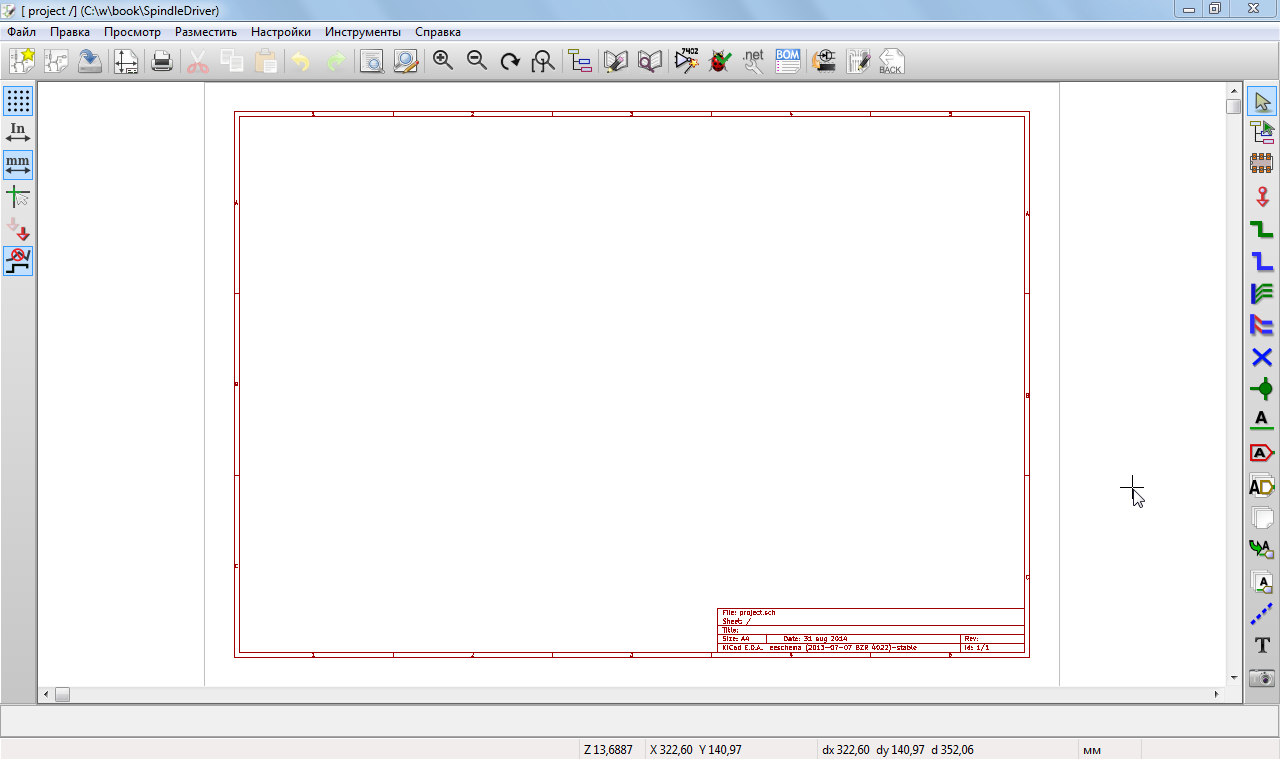
\includegraphics[width=\textwidth]{kicad/ee15.png}

На правом краю окна редактора схем есть вертикальная панель инструментов,
которые мы и будем использовать для рисования схемы. Этими инструментами можно
выбирать объекты, размещать компоненты, вводить связи и т.д.
